\chapter{绪论}\label{chapter_introduction}
\section{研究背景}
在安卓应用中,服务(Services)和广播(Broadcast)得到了广泛的使用。服务可以在安卓应用的后台保持长期运行,提供诸如下载、数据更新等重要功能。然而,正因为服务长期运行于后台的特点,使其往往容易产生异常(Errors)。如果服务的编写人员缺少警惕性,服务中出现的错误(Bug)可能会导致诸多问题,严重者可能引起应用崩溃,甚至系统死机;广播可以实现跨应用通信,要接收来自系统或者其他应用的广播,应用需要编写广播接收器(Broadcast Receiver),广播接收器将在UI线程运行,因此不适合进行耗时操作,通常会在广播接收器中启动服务来进行后续的处理,因此广播接收器也可能通过服务或者自身导致内存泄漏。

安卓应用中的内存泄露指资源(内存对象、句柄、服务等)将不再被使用,但却无法被垃圾回收机制(GC)回收,同时也是服务中的一大类常见问题。服务如果出现内存泄露,将会导致内存使用量意外大幅度增加,进而使得系统效率降低,严重影响用户体验。

服务如果设定'exported:true',则该服务可以被其他应用所调用,因此内存泄露的问题将会变得更加复杂。

由于在安卓8及更高的版本下,安卓操作系统的“电池优化策略”禁止跨应用启动后台服务,而这一方式在安卓7以及更早的版本中是可行的,因此在新版本的安卓系统中,公开服务的内存泄漏检测方法与之前的方法\cite{jun2018lesdroid}有所差别,也正因为禁止跨应用启动后台服务,公开服务的内存泄漏问题也得到了很大的规避。

%\begin{figure}[htbp]
%   \centering
%   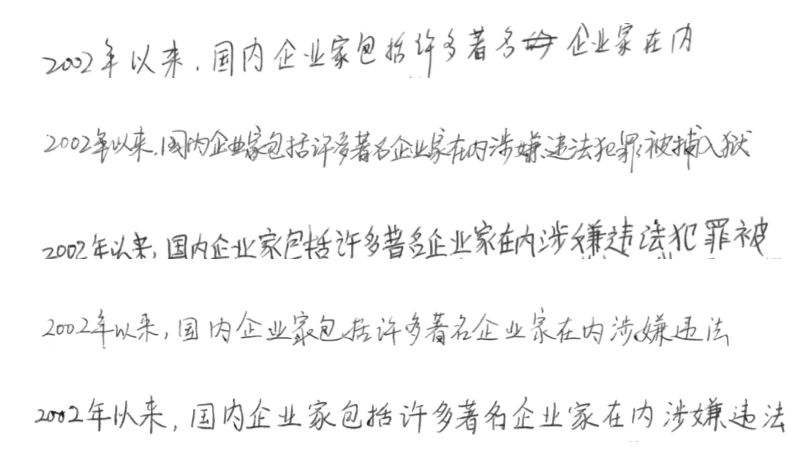
\includegraphics[width=0.9\textwidth]{style.png} % requires the graphicx package
%   \caption{不同的书写风格。对于同一句话,有不同的书写风格:倾斜,写错字,工整,潦草等。}
%   \label{fig:style}
%\end{figure}

\section{相关工作}

Erika 等人在安卓8之前的版本中,编写了一个检测跨应用通信安全问题的工具Com Droid\cite{chin2011analyzing},文中阐述的方法对于跨应用测试具有指导意义。


在安卓8之前的版本中,跨应用启动服务这一行为是被允许的,南京大学的马骏等人安卓8之前的版本中,实现过一个公开服务(Exported Services)内存泄漏的检测工具LES Droid\cite{jun2018lesdroid},文中采用的方式分为四步:

\begin{enumerate}
	\item 使用apktool反编译工具\cite{apktool}获取被测试应用的AndroidManifest.xml文件,解析获取应用中所有的公开服务的包名和类名。
	\item 将测试驱动应用、被测试应用通过adb安装到模拟器中,启动测试驱动应用。
	\item 测试驱动应用重复启动、关闭被测试的服务,在满足一定测试强度之后,导出被测试应用的堆镜像文件(.hprof files)。
	\item 基于MAT内存分析库\cite{mat}编写堆镜像文件的分析工具,自动检测内存泄漏并统计泄露的入口等。
\end{enumerate}


文中的数据指出:在41537个被测试应用中,共在其中28662(69\%)个应用中检测出74831个服务,其中3934(13.7\%)个应用拥有公开服务。经过去重、安装测试以及应用商店评分筛选,有375个实际测试应用,最终通过不同的测试配置,最终检测到在18.7\%的应用中有16.8\%的服务存在内存泄漏问题。


\section{本文主要工作}
本文旨在探索一套适用于安卓8以上版本的公开服务和静态注册广播接收器的内存泄漏检测方法。主要工作如下:
\begin{enumerate}
\item 找到在安卓8以上版本的安卓系统上可行的跨应用测试方法。

\item 对桩应用上进行测试,并能发现所有泄露。

\item 在应用商店中下载真实应用,进行自动化测试分析实验结果。

\end{enumerate}
\section{本文结构}
本文的各章节组织结构如下:
\begin{itemize}
	\item[第一章] 绪论。简要说明了安卓组件内存泄漏的现象和后果。并概括地描述了检测安卓不可见控件内存泄漏的方法流程,总结了本文结构。
	\item[第二章] 自动化检测工具。
	\item[第三章] 实验。介绍了实验进行的配置环境,测试使用应用的来源,以及实验数据结果。
	\item[第四章] 总结与讨论。总结全文工作,讨论存在的问题和今后可以继续研究的方向。
\end{itemize}